\chapter{Kajian Pustaka}
Untuk mendirikan landasan berfikir, bab ini akan membahas fakta dan teori yang berkaitan dengan perancangan sistem tersebut. Dimulai dengan membahas beberapa riset terkait, dilanjutkan dengan penjelasan akan istilah istilah, dan algoritma yang digunakan pada penerapan tugas akhir pada bab 3.

\section{Penelitian terkait monitoring aritmia}
\textit{Monitoring} jantung bukanlah hal yang baru. Hal ini ditandai dengan banyaknya produk dan riset mengenai \textit{monitoring} jantung. Sebelum berdiskusi lebih jauh tentang riset terkait aritmia ada baiknya penulis mereview beberapa produk terkait monitoring jantung yang ada dipasaran.

\subsection{Produk Monitoring Jantung di Pasaran}
Meningkatnya kesadaran masyarakat akan CVDs mendorong banyak perusahaan untuk membuat produk \textit{monitoring} jantung \textit{portable}. Perusahaan seakan berlomba memproduksi alat monitoring baik yang berstandar medis untuk penggunaan rawat intesif maupun yang tidak berstandar medis untuk penggunaan sehari hari. Selain produk berbentuk alat (\textit{hardware}), produk berbentuk program (\textit{software}) yang hanya memanfaatkan \textit{LED flash} di kamera \textit{smartphone} sebagai sensor PPG juga banyak ditemukan \cite{playstore_heart}.

Salah satu perusahaan yang ikut memproduksi alat \textit{monitoring} ialah perusahaan yang terkenal dengan jam tangan pintarnya yaitu Fitbit. Fitbit mengeluarkan ``Fitbit Blaze" pada tahun 2016 \cite{online:fitbit}. Fitbit Blaze dilengkapi dengan PPG pada bagian belakangnya. Fitbit Blaze juga dilengkapi aplikasi Android untuk melihat hasil \textit{monitoring} secara lengkap. Fitbit Blaze terhubung kepada ponsel Android menggunakan Bluetooth. Fitbit Blaze dirancang sebagai pelengkap \textit{lifestyle} agar penggunanya dapat menggunakannya sehari hari. Hasil \textit{monitoring} dari Fitbit dapat dibagikan kepada siapapun setelah sebuah \textit{record} selesai direkam.

Sama seperti Fitbit, perusahaan raksasa dari Korea, Samsung, juga mengeluarkan produk \textit{lifestyle} berupa sebuah jam tangan pintar yang dapat melakukan \textit{monitoring} jantung. Produk milik Samsung diberi nama ``Gear S3" (gambar \ref{fig:device_example} a) dan diluncurkan pada tahun 2017 \cite{online:samsung_gear}. Gear S3 dilengkapi sensor PPG di bagian belakangnya. Gear S3 dapat terhubung ke jaringan secara \textit{wireless} dengan menggunakan koneksi \textit{Bluetooth} dan \textit{Wi-Fi}. Hasil \textit{monitoring} dari Gear S3 hanya dapat dilihat pada layar yang melengkapinya.

PT. Endo Indonesia, sebuah perusahaan peralatan medis asal Indonesia, juga membuat alat \textit{monitoring} jantung. Tidak seperti Fitbit dan Samsung, produk besutan Endo ditujukan untuk pemakaian medis. Endo memproduksi Holter monitor ``EDAN SE-2003" (gambar \ref{fig:device_example} b) dan Pulse Oximeter ``EDAN H-10" (gambar \ref{fig:device_example} c). "SE-2003" menggunakan sensor berjenis ECG dan mampu melakukan \textit{monitoring} pada 3 \textit{channel} sekaligus \cite{endo_holter}. Berbeda dengan ``SE-2003", ``H-10" menggunakan PPG \cite{endo_oxi}. Pulse Oximeter ``H-10", sesuai namanya, selain mampu \textit{monitoring} jantung (\textit{Pulse}) juga mampu mengukur kadar oxigen dalam darah (\textit{Oximeter}). ``H-10" merupakan pulse oximeter yang diletakkan pada ujung jari (\textit{fingertip}). Hasil \textit{monitoring} holter monitor dan pulse oximeter Endo dapat dilihat pada layar produk tersebut dan aplikasi desktop yang menyertainya.

Produk berupa aplikasi/\textit{software} (gambar \ref{fig:device_example} d) dapat ditemukan dengan mudah pada toko aplikasi \textit{virtual} (\textit{playstore}, \textit{app store}, dll). Penulis melakukan studi perbandingan terhadap 10 aplikasi teratas (versi Juli 2017) pada daftar hasil pencarian di \textit{Play Store}, dengan kata kunci ``Heart Rate" \cite{playstore_heart}. Setelah membandingkan aplikasi tersebut, tidak ditemukan aplikasi yang memiliki fitur \textit{monitoring} lengkap untuk menyelesaikan permasalahan yang diajukan pada bab sebelumnya. Hasil perbandingan terhadap 10 aplikasi ini dicantumkan pada tabel \ref{table:app_comparison}

Semua produk yang disebutkan sebelumnya tidaklah \textit{Open Source}. Sehingga tidak dimungkinkan untuk merubah spesifikasi kinerja produk seperti menaikkan \textit{sample rate} atau mengganti algorima penghitung detak jantung. Walaupun tidak \textit{Open Source}, baik Fitbit dan Samsung memberikan \textit{Application Programming Interface} (\textit{API}) untuk memudahkan pengembang perangkat lunak membuat sistem yang menggunakan produk mereka. API tersebut memungkinkan pengembang mengambil semua data sensor yang tertanam pada produk. Untuk kasus \textit{monitoring} jantung, pengembang dapat mengambil bentuk gelombang jantung dan BPM dari produk. Sedangkan, Endo tidak menyediakan API sama sekali. Sehingga, untuk mengakses pengukuran dari produk Endo akan sangat sulit untuk dilakukan (mungkin dilakukan dengan \textit{Reverse Engineering}). Rangkuman perbedaan produk berupa alat dapat dilihat pada tabel \ref{table:product_comparison}

\begin{figure}[H]
    \centering
	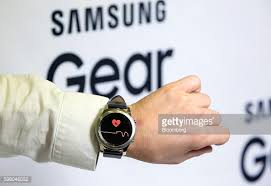
\includegraphics[scale=0.4]{images/gears3.jpg}
	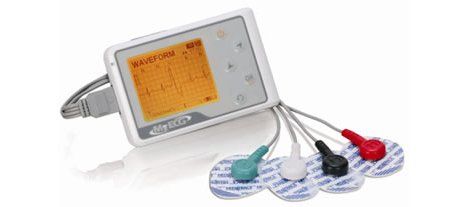
\includegraphics[scale=0.3]{images/ecg_1.jpg}	
	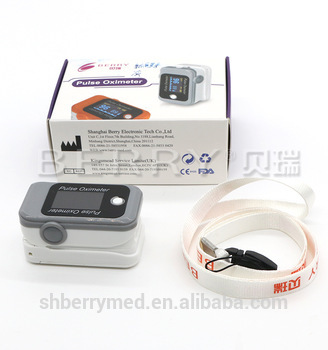
\includegraphics[scale=1]{images/ppg_clip.jpg}
	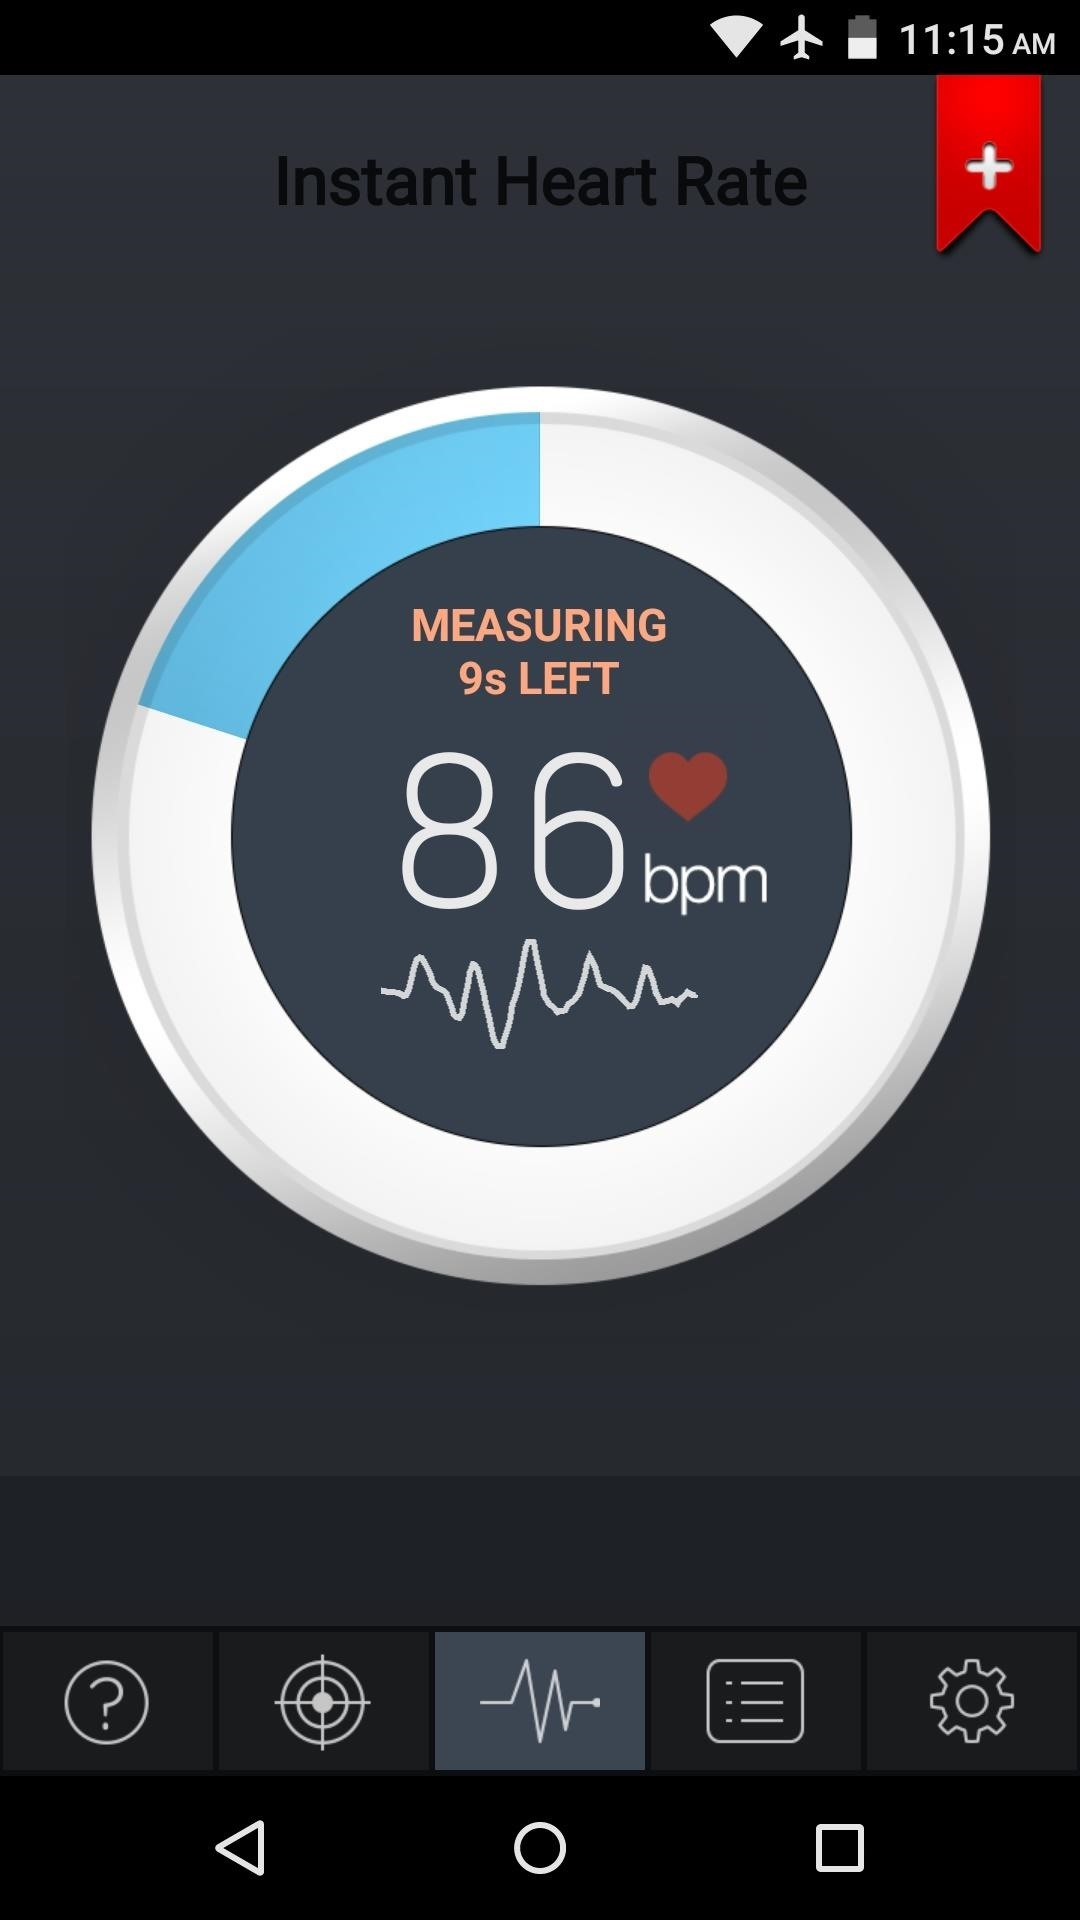
\includegraphics[scale=0.04]{images/heart_app1.jpg}
    \caption{a) Samsung Gear S3; b) Holter Monitor; c) Fingertip Pulse Oximeter; d) Heart Rate App}
    \label{fig:device_example}
\end{figure}

\begin{table}[H]
	\centering
	\begin{tabular}{|l|L{3cm}|c|c|c|L{0.5cm}|L{0.5cm}|L{0.5cm}|L{0.5cm}|L{0.5cm}|L{0.5cm}|L{0.5cm}|L{0.5cm}|}
		\hline
		\rowcolor{gray}
		\textbf{No} & \textbf{Produk} & \textbf{Sen} & \textbf{Me} & \textbf{Op} & \multicolumn{8}{c}{\textbf{Fitur}} \\
		\rowcolor{gray}
		 & & \textbf{sor} & \textbf{dis} & \textbf{en} & A & B & C & D & E & F & G & H \\
		\hline
		1 & Fitbit Blaze & PPG & N & N & Y & Y & Y & Y & N & Y & N & Y \\
		2 & Samsung Gear S3 & PPG & N & N & Y & Y & Y & N & N & Y & N & Y \\
		3 & ENDO SE-2003 & ECG & Y & N & Y & Y & Y & Y & N & Y & N & N \\
		4 & ENDO H-10 & PPG & Y & N & Y & Y & Y & Y & N & Y & N & N \\
		\hline
	\end{tabular}
	\caption{Perbandingan Produk Berupa Alat}
	\label{table:product_comparison}
\end{table}

\begin{table}[H]
	\centering
	\begin{tabular}{|l|L{4cm}|c|L{0.5cm}|L{0.5cm}|L{0.5cm}|L{0.5cm}|L{0.5cm}|L{0.5cm}|L{0.5cm}|L{0.5cm}|}
		\hline
		\rowcolor{gray}
		\textbf{No} & \textbf{Aplikasi} & \textbf{Sen} & \multicolumn{8}{c}{\textbf{Fitur}} \\
		\rowcolor{gray}
		 & & \textbf{sor} & A & B & C & D & E & F & G & H \\
		\hline
		1 & Instant Heart Rate : Heart Rate \& Pulse Monitor & PPG & Y & N & Y & Y & N & Y & N & Y \\
		2 & iCare Health Monitor (BP \& HR) & PPG & Y & N & Y & N & N & Y & N & Y \\
		3 & Heart Rate Monitor(REPS) & PPG & Y & N & Y & Y & N & Y & N & Y \\
		4 & Runtastic Heart Rate Monitor \& Pulse Checker & PPG & Y & N & Y & N & N & Y & N & N \\
		5 & Cardiograph - Heart Rate Meter & PPG & Y & N & Y & Y & N & Y & N & Y \\
		6 & ASUS Heart Rate & PPG & N & N & N & N & N & Y & N & N \\
		7 & Samsung Health & PPG & Y & Y & N & N & N & Y & N & Y \\
		8 & Heart Rate Monitor(Meet Your Need Production) & PPG & N & N & N & N & N & Y & N & N \\
		9 & \textbf{MobECG} & \textbf{ECG} & N & Y & Y & Y & N & Y & N & N \\		
		10 & \textbf{CMS50Dplus} & \textbf{ECG} & N & Y & Y & Y & N & Y & N & N \\
		\hline
	\end{tabular}
	\caption{Perbandingan 10 Aplikasi Monitoring Jantung di Play Store}
	\label{table:app_comparison}
\end{table}

Ket: \\
A = Identitas User \\
B = Real Time Monitoring \\
C = Melihat Gelombang Jantung \\
D = Merekam Gelombang Jantung \\
E = Multiuser Monitoring \\
F = Deteksi BPM \\
G = Aritmia Alert \\
H = Share Result via Network \\

\subsection{Riset Terkait}
Arsitektur sistem yang dirancang pada tugas akhir ini menerapkan konsep Internet of Things (IoT) dan diharapkan mampu melakukan analisis otomatis, khususnya aritmia. Penerapan IoT kedalam \textit{monitoring} jantung sudah pernah dilakukan sebelumnya, begitupun dengan analisis artimia secara otomatis. Untuk mengoptimalkan metode yang diajukan pada tugas akhir ini, diperlukan pembelajaran terhadap riset terkait atas kedua hal tersebut.

Pada tahun 2013, Daniel Barata dan rekannya dari Portugal merancang metode \textit{monitoring} yang dapat bekerja secara \textit{portable} \cite{daniel_barataa}. Sensor yang terhubung dengan sebuah tablet android akan berkomunikasi menggunakan protokol MQTT. Penggunaan MQTT memungkinkan \textit{throughtput} data yang besar dan banyak sensor yang terhubung secara bersamaan. Metode ini menggunakan sensor ECG dan PPG untuk mengambil data tubuh. Pemilihan MQTT untuk meningkatkan jumlah sensor yang dapat terhubung juga dilakukan oleh Karan Motwani pada penilitiannya di tahun 2016 \cite{karan_motwani}. Selain digunakan untuk \textit{monitoring} MQTT juga digunakan pada \textit{facebook messager} \cite{mqtt_use}.

Pada tahun 2014, Paola Pierleoni dan rekannya merancang metode monitoring yang melibatkan ponsel dan sensor ECG milik produk ``Zephyr HxM-BT" \cite{paola_pierleoni}. Zephyr akan mengirimkan sinyal ECG melalui bluetooth menuju polsel untuk di proses. Metode \textit{monitoring} yang dirancang oleh Pierleoni menambahkan analisis aritmia kedalamnya. Aritmia dianalisis menggunakan \textit{rule based classification} yang diusulkan oleh Tsipouras(2005). Aturan yang diajukan oleh Tsipouras memerhatikan fitur RR interval dari gelombang jantung \cite{rr_classification}. Hasil analisis yang dihasilkan dapat dilihat secara \textit{real time} pada layar ponsel.

Pada tahun 2015, M. Surya dan rekannya asal India merancang arsitektur \textit{monitoring} jantung yang dibangun menggunakan Raspberry Pi \cite{surya}. Sebuah ECG akan memberikan inputan analog kepada pin GPIO yang dimiliki oleh Raspi. Raspi bertugas untuk mendeteksi detak jantung dan mengirimkan perhitungan BPM ke sebuah \textit{dashboard} melalui jaringan GSM. Setiap data gelombang jantung yang diterima \textit{dashboard} akan disimpan pada database MySQL.

Masih di tahun 2015, Naresh Vemishetty dan rekannya merancang metode \textit{monitoring} yang ditujukan agar memiliki kompleksitas pemrosesan yang rendah \cite{naresh}. Dengan kompleksitas yang rendah diharapkan metode yang mereka usulkan ini dapat dijalankan pada device yang memiliki kemampuan komputasi yang rendah. Sistem mereka dapat menerima input berupa sinyal ECG dan EEG.

Pada tahun 2016, Vasu Jindal (seorang peneliti dari Universitas Texas) merancang metode \textit{monitoring} yang melibatkan penggunaan ponsel dan \textit{cloud}\cite{vasu_jindal}. Ponsel akan membaca gelombang jantung dari sensor PPG milik produk sejenis Fitbit, kemudian mengirimkannya ke \textit{cloud} untuk di proses. \textit{Cloud} akan memprosesnya menggunakan \textit{deep belief network} dan mengembalikan hasil pengukuran berupa BPM. Setiap data gelombang jantung yang diterima \textit{cloud} akan disimpan sebagai bahan prediksi berikutnya.

Di tempat lain pada tahun 2016, Mamidi Manisha dan rekannya dari India merancang metode \textit{monitoring} yang mirip dengan metode Jindal. Metode Mamidi juga melibatkan ponsel, produk jam tangan pintar dan \textit{cloud processing}\cite{mamidi}. Namun fokus utama dalam sistem yang mereka rancang ialah tentang bagaimana cloud dapat menangani pertukaran data yang besar dan cepat. Salah satu kunci keberhasilan sistem mereka ialah penerapan \textit{database} No-SQL yang berhasil memaksimalkan kecepatan penulisan data. Selain komunikasi yang cepat, sistem mereka dirancang agar memiliki mekanisme pemberitaan darurat kepada rumah sakit.

Dari keempat riset diatas, masing masing memiliki kelebihan dan kekurangan. Metode Barata dan Motwani dapat menghubungkan banyak sensor sekaligus. Metode Pierloeni dapat medeteksi aritmia tapi hanya pasien yang bisa mengetahuinya. Metode Jindal memiliki sistem analisis terpusat sehingga algoritma yang diterapkan dapat terus berkembang semakin akurat namun hanya bisa menganalisis BPM. Metode Manisha memiliki kehandalan dalam menangani banyak pasien dalam sistem terpusat dan mampu memberikan pemberitaan darurat namun analisis masih harus dilakukan manual. Ringkasan mengenai kelebihan dan kekurangan ini dapat dilihat pada tabel \ref{table:monitoring_compare}.

\begin{table}[H]
	\begin{tabular}{|L{5cm}|L{3cm}|C{1cm}|c|c|c|c|c|}
		\hline
		\rowcolor{gray}
		\textbf{Judul} & \textbf{Penulis} & \textbf{Ta} & \multicolumn{5}{c}{\textbf{Fitur}} \\
		\rowcolor{gray}
		 & & \textbf{hun} & A & B & C & D & E \\
		 System of acquisition, transmission, storage and visualization of Pulse Oximeter and ECG data using Android and MQTT & Daniel Barata, Goncalo Louzada et al. & 2013 & N & N & N & Y & N \\
		\hline
		 An Android-Based Heart Monitoring System for the Elderly and for Patients with Heart Disease & Paola Pierleoni, Luca Pernini, et al. & 2014 & Y & Y & N & N & Y \\
		\hline
		 Healthcare based on IoT using Raspberry Pi & M. Surya Deekshith Gupta, Vamsikrishna Patchava, et al. & 2015 & Y & N & N & N & Y \\
		\hline
		 Affordable Low Complexity Heart/Brain Monitoring Methodology for Remote Health Care & Naresh Vemishetty, Pranit Jadhav, et al. & 2015 & Y & N & N & N & N \\
		\hline
		Integrating Mobile and Cloud for PPG Signal Selection to Monitor Heart Rate During Intensive Physical Exercise & Vasu Jindal & 2016 & Y & N & Y & N & N \\
		\hline
		IoT on Heart Attack Detection and Heart Rate Monitoring & Mamidi Manisha, Katakam Neeraja, et al. & 2016 & N & N & Y & Y & Y \\
		\hline
	\end{tabular}
	\caption{Perbandingan Riset Metode Monitoring}
	\label{table:monitoring_compare}
\end{table}

Ket: \\
A = Deteksi BPM \\
B = Deteksi Artimia \\
C = Sistem Deteksi Cloud \\
D = Optimasi banyak pengguna \\
E = Sistem Peringatan \\

Analisis terhadap rekam jantung umumnya dilakukan secara manual oleh dokter jantung. Salah satu bentuk analisis yang dapat dilakukan ialah mengklasifikasian kemunculan aritmia. Untuk mengklasifikasikan aritmia seorang dokter perlu melihat hasil rekam jantung seorang pasien (gambar \ref{fig:contoh_aritmia}), baik hasil rekam ECG maupun PPG. Namun, seperti yang ditunjukkan oleh Pierleoni (2014) pada penilitiannya dimungkinkan untuk melakukan analisis otomatis, khususnya Aritmia \cite{paola_pierleoni}. Selain Pierleoni, banyak penelitian yang telah dilakukan untk mengklasifikasi aritmia secara otomatis. Bahkan, kini penelitian tersebut telah memiliki keakuratan yang cukup baik, mencapai lebih dari 90\%, dengan berbagai macam metode dan ekstraksi fitur.

Pada tahun 1985, Jiapu Pan dan Willis J. Tompkins mengusulkan sebuah metode deteksi QRS secara \textit{Real Time} \cite{pantom}. Metode ini kemudian menginspirasi peneliti lainnya untuk menerapkannya ke dalam berbagai penelitian mengenai \textit{monitoring} jantung \cite{pantom_hardware, pantom_hardware2}. Salah satu peneliti yang menggunakan metode ini ialah Christos Pavlatos dan rekannya pada tahun 2003 \cite{pantom_hardware}. Christo Pavlatos menerapkan metode Pan dan Tompkins kedalam \textit{embedded system}. Hal ini dimungkinkan karena algoritma pan tompkins cukup hemat dalam penggunaan memori, panjang buffer yg digunakan yaitu 150ms. Algoritma Pan dan Tompkins berhasil mendeteksi detak jantung dengan tingkat sensitivitas 99.62\% \cite{pantom}.

Pada tahun 2004, Tsipouras dan rekannya mengajukan algoritma klasifikasi aritmia berdasarkan RR-interval \cite{rr_classification}. Klasifikasi yang diajukan berupa \textit{rule-based} yang dirancang bersama dokter ahli jantung. Algoritma yang dianggap simpel dibandingkan penggunaan algoritma \textit{machine learning} seperti SVM \cite{aritmia_svm}, ANN \cite{aritmia_ann}, dan Regressor. Algoritma ini menghasilkan akurasi 98\%.

Pada tahun 2008, Babak Mohammadzadeh dan rekannya mengajukan algoritma yang dapat mendeteksi aritmia menggunakan \textit{Generalized discriminant analysis} (GDA) dan \textit{Support Vector Machine} (SVM) \cite{aritmia_svm}. Algoritma yang diusulkan Mohammadzadeh mampu mengklasifikasikan NSR, PVC, AF, VF and 2$^{\circ}$ Heart Block pada sinyal ECG. Algorima yang diusulkan Mohammadzadeh menghasilkan akurasi 99.1\%.

Pada tahun 2013, Milan S. Shet dan rekannya mengajukan metode klasifikasi aritmia dengan input ECG \cite{aritmia_swarm}. Algoritma mereka melibatkan optimasi \textit{Binary Particle Swarm} dan \textit{Absolute Euclidean Classifier}. Metode Shet menghasilkan akurasi 97.2\%.

Pada tahun 2014, Andrius Solosenko dan Vaidotas Marozas mengajukan metode yang dapat mendeteksi PVC (tipe aritmia) yang menggunakan inputan PPG \cite{aritmia_ann}. Algoritma deteksi yang diterapkan menggunakan klasifikasi \textit{artificial neural network} (ANN) dengan 6 fitur pada 12 detik \textit{window}. Algoritma ini menghasilkan spesitivitas 99.85\%.

Pada tahun 2015, Luisa F. Polania dan rekannya mengajukan metode klasifikasi aritmia dengan menerima input PPG \cite{aritmia_svm_ppg}. Tipe aritmia yang dapat diklasifikasi ialah NSRs, \textit{paced} SVPCs, \textit{paced} VPC dan \textit{paced} VT. SVM digunakan sebagai klasifikasi atas 3 fitur. Algortima yang mereka ajukan memiliki akurasi 96\%.

Pada tahun 2016, Kalidas dan Tamil mengajukan algoritma klasifikasi aritmia yang dapat memproses 3 jenis input, ECG, PPG, dan \textit{Arterial Blood Pressure} (ABP) \cite{ecg_syncro}. Sinyal ECG diproses menggunakan algoritma Pan-Tompkin dan PPG diproses menggunakan "first-order derivative" filter. Klasifikasi yang digunakan kombinasi dari \textit{adaptive threshold} dan SVM. Algoritma yang mereka ajukan menghasilkan spesitivitas 96\%

Ringkasan dari hasil keenam riset diatas dapat dilihat pada tabel \ref{table:analysis_compare}.

\begin{table}[htbp]
\centering
	\begin{tabular}{|L{4cm}|L{2.5cm}|C{1cm}|L{4cm}|L{1cm}|}
	\hline
	\rowcolor{gray}
	\textbf{Judul} & \textbf{Penulis} & \textbf{Tahun} & \textbf{Hasil} & \textbf{Sensor} \\
	\hline
	An arrhythmia classification system based on the
RR-interval signal & M.G. Tsipouras, D.I. Fotiadis, \textit{et al} & 2004 & Algoritma klasifikasi aritmia dengan fitur RR interval dan rule-base decision & ECG \\
	\hline	
	Support vector machine-based arrhythmia classification using reduced features of heart rate variability signal & Babak Mohammadzadeh Asl, Seyed Kamaledin Setarehdan, \textit{et al} & 2008 & Model klasifikasi aritmia berdasar GDA dan SVM & ECG \\
	\hline
	ECG Arrhythmia Classification Using R-Peak Based Segmentation, Binary Particle Swarm Optimization and Absolute Euclidean Classifier & Milan S. Shet, Minal Patel, \textit{et al} & 2013 & Model particle swarm yang mengkalsifikasi segmen R peak & ECG \\
	\hline
	Automatic Premature Ventricular Contraction Detection in Photoplethysmographic Signalsr & Andrius Solosenko and Vaidotas Marozas & 2014 & Algoritma deteksi PVC pada sinyal PPG & PPG \\
	\hline
	Method for Classifying Cardiac Arrhythmias using Photoplethysmography & Luisa F. Polania, Lalit K. Mestha, \textit{at al} & 2015 & Algoritma deteksi arimia berdasarkan 3 fitur PPG & PPG \\
	\hline
	Cardiac arrhythmia classification using multi-modal signal analysis & V Kalidas and L S Tamil & 2016 & Metode klasifikasi aritmia dengan kombinasi input ECG dan PPG & ECG, PPG \\
	\hline
	\end{tabular}
	\caption{Ringkasan riset mengenai klasifikasi aritmia otomasis}
	\label{table:analysis_compare}
\end{table}

\section{ECG dan PPG}
Terdapat 2 jenis sensor yang umum digunakan untuk melakukan \textit{monitoring} jantung, yaitu \textit{Electrocardiogram} (ECG) dan \textit{Photoplethysmogram} (PPG) seperti yang terlihat pada gambar \ref{fig:ecg_n_ppg}. Kedua jenis sensor ini menjadi pilihan utama dalam \textit{monitoring} jantung karena keduanya mengusung konsep \textit{non-invasive}. Sensor non-invasive memungkinkan melakukan pengambilan data tubuh tanpa perlu melukai/menusuk bagian tubuh tertentu. Secara umum ECG akan menghasilkan pengukuran lebih akurat dari pada PPG. Namun PPG lebih nyaman digunakan dalam jangka panjang dari pada ECG.

\begin{figure}[H]
    \centering
    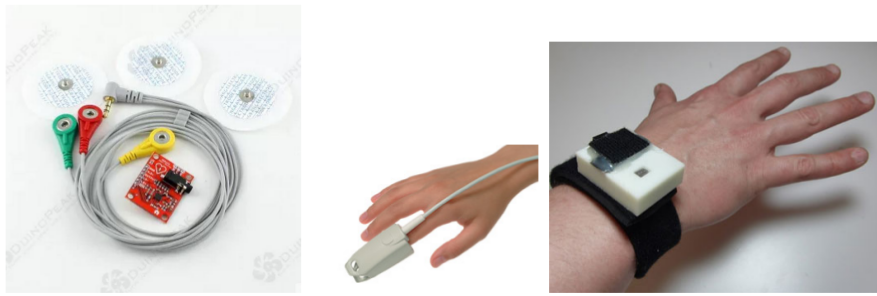
\includegraphics[scale=0.3]{images/sensors.png}
    \caption{a) Sensor ECG dengan 3 \textit{leads}; b) Sensor PPG ujung jari; c) Sensor PPG di pergelangan tangan}
    \label{fig:ecg_n_ppg}
\end{figure}

\subsection{Lokasi Penempatan Sensor}
\subsubsection{a. ECG}
ECG perlu melakukan pengukuran minimal di 3 lokasi. Hal ini disebabkan karena ECG secara langsung mengukur perubahan nilai kelistrikan yang dihasilkan tubuh. Untuk mengukur kelistrikan tubuh ECG memerlukan minimal 3 elektroda yaitu + (positif), - (negatif) dan N (netral), terlihat pada gambar \ref{fig:electrode3}. Untuk pengukuran lebih dari 3 titik, elektroda ECG dapat diletakkan pada posisi yang ditunjukkan gambar \ref{fig:multi_elctrode}.

\begin{figure}[H]
    \centering
    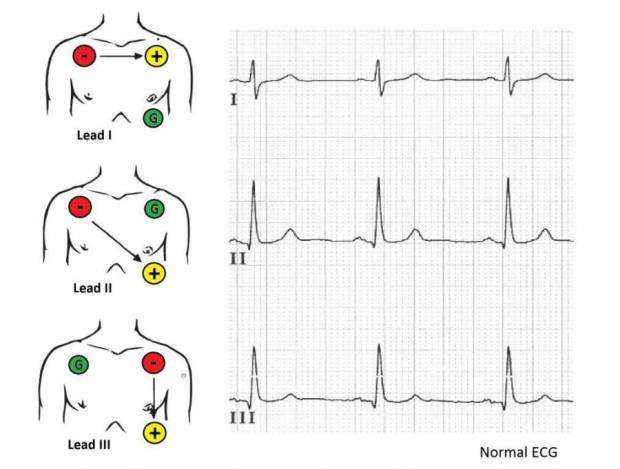
\includegraphics[scale=0.3]{images/3_ecg_place.jpg}
	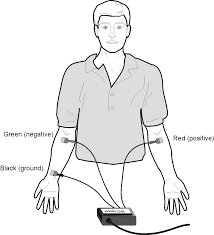
\includegraphics[scale=0.6]{images/3_ecg_place_2.png}    
    \caption{a) Penempatan 3 Elektroda di Dada, b) Penempatan 3 Elektroda di Tangan}
    \label{fig:electrode3}
	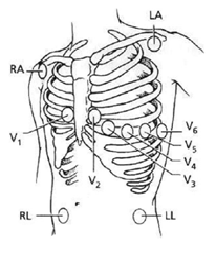
\includegraphics[scale=0.8]{images/multi_ecg.png}
    \caption{Lokasi Penempatan Lebih 3 titik}
    \label{fig:multi_elctrode}
\end{figure}

\subsubsection{b. PPG}
PPG dapat melakukan pengukuran hanya di satu lokasi. Hal ini disebabkan karena PPG mengukur tingkat penyerapan cahaya oleh darah, sedangkan pembuluh darah menjalar ke seluruh tubuh. Namun, untuk menghasilkan pengukuran maksimal PPG perlu diletakkan di lokasi tubuh yang pembuluh darah dekat dengan permukaan kulit \cite{ppg_placement}\cite{ppg_placement2}. Beberapa lokasi tubuh yang sesuai kriteria tersebut terdapat pada ujung jari, pergelangan tangan, lengan atas, leher, dan daun kuping.


\subsection{Titik Fiducial}
Untuk mengenali sebuah detak jatung pada rekam ECG maupun PPG diperlukan untuk mencari titik titik \textit{fiducial} (pembanding). Kemunculan titik fiducial menandakan adanya siklus \textit{beat} (detak) pada waktu kemunculan titik tersebut. Sebuah siklus sinyal ECG dapat dilihat dari beberapa titik fiducial yaitu P-QRS-T, seperti terlihat pada gambar \ref{fig:ecg_points}. Sedangkan siklus sinyal PPG dilihat dari siklus Diastolic-Systolic-Dicrotic seperti terlihat pada gambar \ref{fig:ppg_points}

\begin{figure}[H]
    \centering
    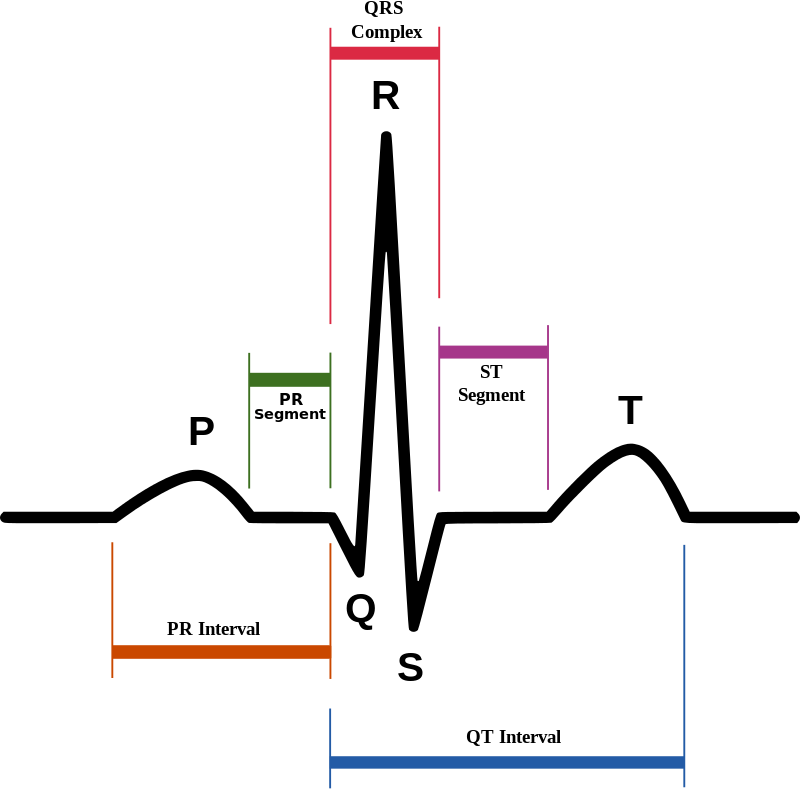
\includegraphics[scale=0.2]{images/ecg_points.png}
    \caption{Sinyal ECG berdasarkan titik fiducial}
    \label{fig:ecg_points}
	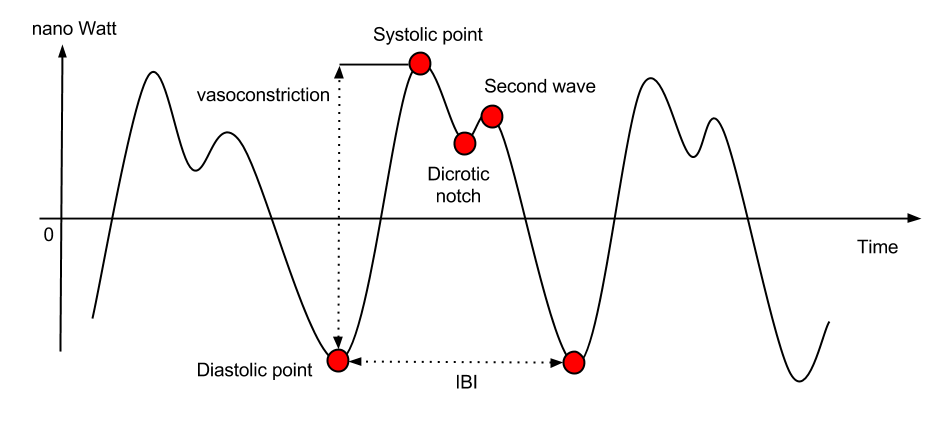
\includegraphics[scale=0.3]{images/PPG2.png}
    \caption{Sinyal PPG berdasarkan titik fiducial}
    \label{fig:ppg_points}
\end{figure}


\subsection{Bentuk Sinyal}
Dapat dilihat, pada gambar \ref{fig:ecg_vs_ppg}, dengan mudah bahwa sinyal bentukan dari PPG dengan ECG berbeda secara morfologi (bentuk)\cite{ppg_vs_ecg}. Namun, karena sumber sinyal yang sama (dari jantung) siklus PPG dan ECG dapat disinkronisasi (saling dipetakan) berdasarkan titik R pada ECG dan puncak sistolik pada PPG seperti gambar \ref{fig:ecg_vs_ppg2} \cite{ecg_syncro}. Perbedaan waktu kemunculan R dan Sistolik dikenal sebagai \textit{Pulse Arrival Time} (PAT). PAT dapat digunakan sebagai parameter mengukur tekanan darah, yang mana tidak dicakup pada tugas akhir ini.

\begin{figure}[H]
    \centering
    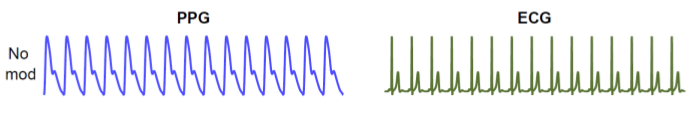
\includegraphics[scale=0.6]{images/ecg_vs_ppg.png}
    \caption{Perbandingan sinyal ideal PPG dan ECG}
    \label{fig:ecg_vs_ppg}
	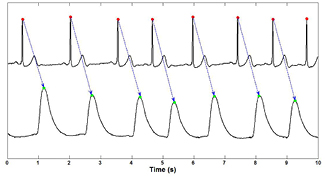
\includegraphics[scale=0.8]{images/sinkronisasi.jpg}
    \caption{Sinkronisasi antara ECG dan PPG}
    \label{fig:ecg_vs_ppg2}
\end{figure}

\section{Aritmia}
Aritmia adalah kategori gangguan jantung yang berupa tidak normal-nya irama jantung. Beberapa panyakit jantung yang tergolong aritmia antara lain:
\begin{itemize}
	\item \textit{Tachycardia} (detak lebih cepat dari normal),
	\item \textit{Bradycardia} (detak lebih lambat dari normal),
	\item \textit{Premature Atrial Contraction} (PAC), Kontraksi Atrial Prematur (gambar \ref{fig:contoh_aritmia} b);
	\item \textit{Premature Vantricular Contraction} (PVC), Kontraksi Ventrikular Prematur (gambar \ref{fig:contoh_aritmia} c);
	\item \textit{Ventricular Tachycardia} (VT) (detak ventrikel sangat cepat), dan
	\item \textit{Ventricular Fibrillation} (VF), detak ventrikel tidak beraturan (gambar \ref{fig:contoh_aritmia} a).
\end{itemize}

\textit{Premature Contraction} berarti siklus detak yang \textit{premature} (tidak pada waktunya) disebabkan oleh kontraksi pada atrium (bilik) atau ventrikel (serambi) terjadi lebih cepat atau lebih lambat dari seharusnya. \textit{Premature Contraction} tergolong serangan kecil (tidak berbahaya)[xx], sedangkan VT dan VF tergolong serangan besar (berbahaya). \textit{Premature contraction} yang terjadi berulang kali dan cepat merupakan awal dari peristiwa VT maupun VF. Contoh kemunculan PAC, PVC dan VF dapat dilihat pada gambar \ref{fig:contoh_aritmia}.

\begin{figure}[H]
    \centering
    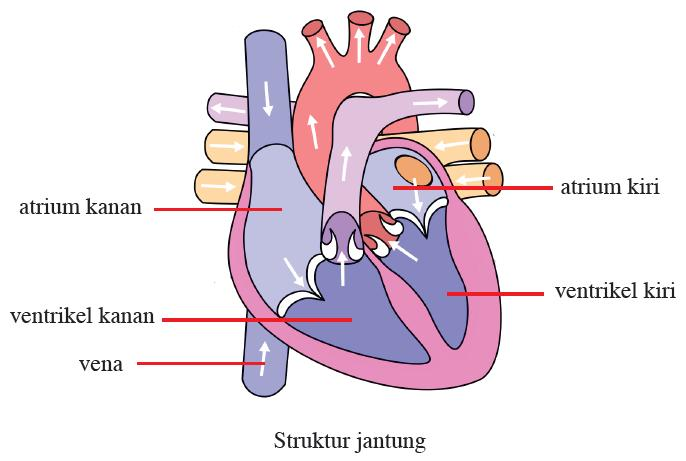
\includegraphics[scale=0.4]{images/jantung.jpg}
    \caption{Struktur jantung sederhana}
	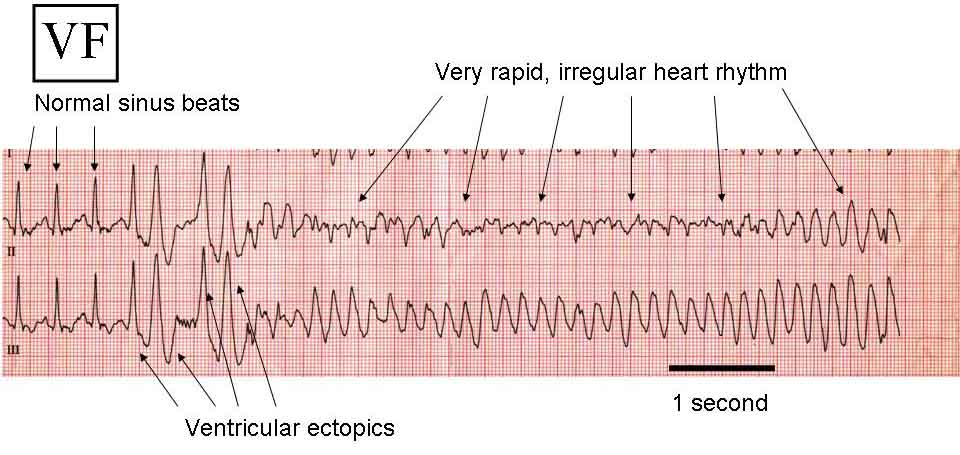
\includegraphics[scale=1.2]{images/VF.jpg}
    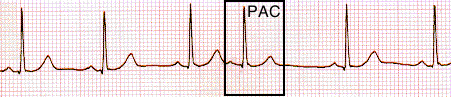
\includegraphics[scale=0.5]{images/PAC1.png}
	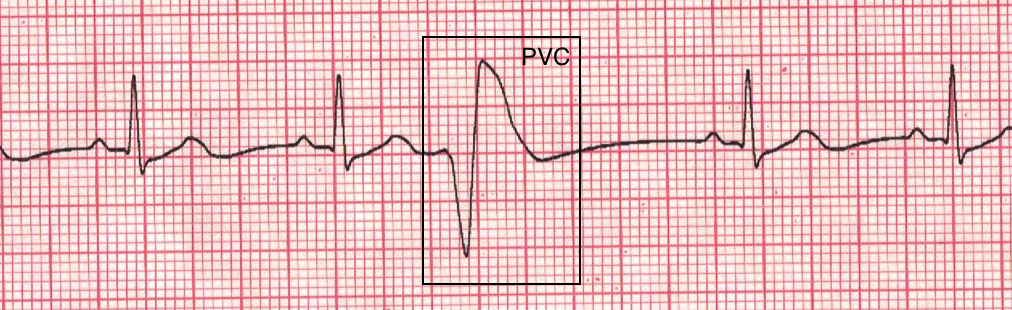
\includegraphics[scale=0.25]{images/PVC1.png}
    \caption{a) Sinyal VF; b) Sinyal PAC; c) Sinyal PVC}
    \label{fig:contoh_aritmia}	
\end{figure}


\section{Internet of Things}
\textit{Internet of Things} (IoT) ialah konsep dimana objek objek (Things) dapat saling berinteraksi pada jaringan Internet tanpa membutuhkan manusia. Pada konsep IoT, terdapat sedikitnya 3 komponen dalam aristekturnya yaitu \textit{sensor}, \textit{server} dan \textit{actuator}. \textit{Sensor} sebagai pengubah data dari dunia nyata ke bentuk digital agar dipahami oleh mesin. \textit{Server} sebagai pemroses data tersebut. Actuator sebagai pelaksana keputusan sensor di dunia nyata. IoT memungkinkan komunikasi \textit{Machine to Machine} (M2M) terjadi dalam jaringan Internet. Hal ini berarti \textit{sensor}, \textit{server} dan \textit{receptor} dapat berkomunikasi dimana saja selama dapat terhubung dengan Internet. Selain itu, IoT memodelkan jaringan agar banyak objek (\textit{Things}) dapat saling berkomunikasi. Sehingga, sebuah sistem yang dirancang untuk menangani banyak objek saling berkomunikasi dimana saja, perlu menerapkan IoT.

Sebuah sistem monitoring yang dapat berjalan secara Ubiquitous haruslah dibangun dengan konsep \textit{Internet of Things} (IoT). Sensor yang berfungsi sebagai pengambil data dikendalikan oleh sebuah \textit{controller}. \textit{Controller} adalah bagian yang mengatur jadwal pengambilan data sensor dan pengirimannya ke server. Salah satu jenis controller yang popular ialah ESP-12. Server memerlukan sebuah platform pemograman yang dapat mengatur pemrosesan data dan komunikasi benda di jaringan. Platform server yang populer untuk penerapan IoT adalah Node.JS. Selain melayani komunikasi, server juga bertugas untuk menyimpan data. Mongo.Db adalah salah satu \textit{database} NoSQL yang populer untuk digunakan dalam sistem yang menyimpan \textit{big data}.

\subsection{ESP-12}
ESP-12 (subversi ESP8266) adalah salah satu tipe \textit{System on Module} (SoC) yang diproduksi oleh Espressif dari China. SoC berarti papan sirkuit yang telah terintegrasi oleh sistem tertentu. Kelebihan utama ESP ialah ukurannya yang kecil (16x24x3 mm) tapi dapat berfungsi sebagai \textit{controller} dan telah dilengkapi modul Wi-Fi. Hal ini memungkinkan komunikasi sensor-server melalui jaringan WiFi tanpa perlu menambah modul jaringan lagi.

\begin{figure}[H]
	\centering
	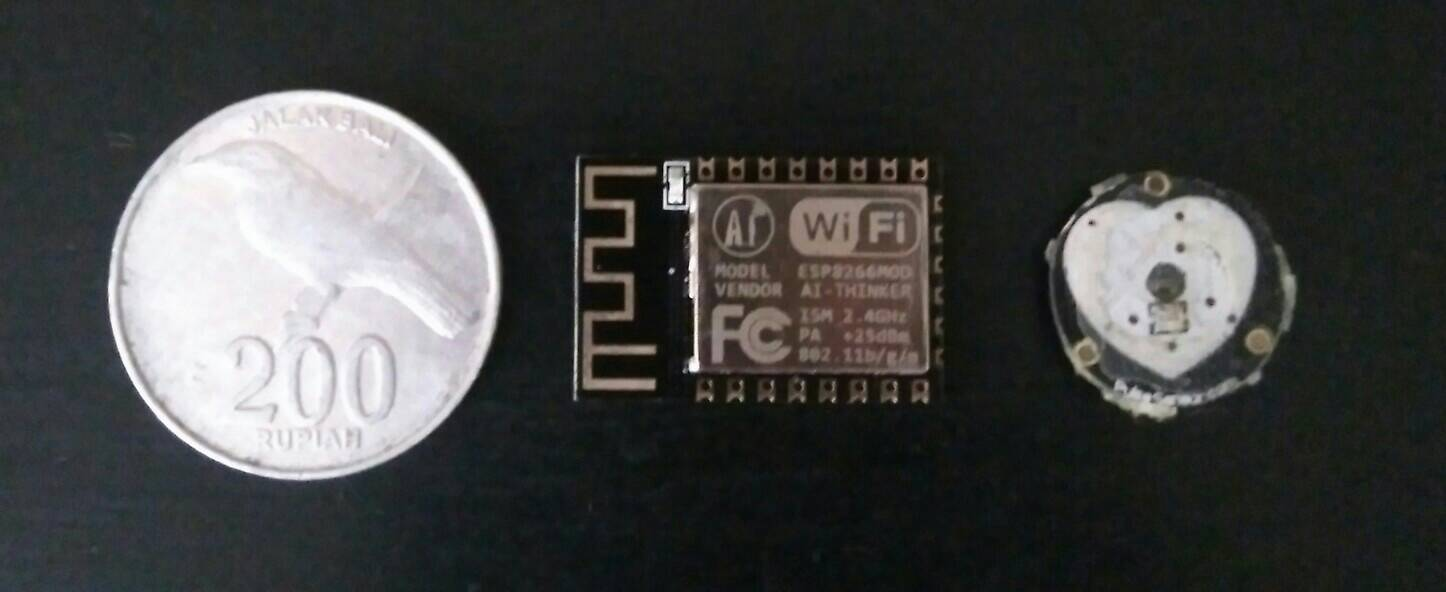
\includegraphics[scale=0.22]{images/coin_esp_pulse.jpg}
	\caption{Koin Rp200 - ESP-12E - Pulse Sensor}
	\label{fig:coin_esp_pulse}
\end{figure}

\subsection{Node.Js}
Node.Js adalah teknologi Javascript (Js) \textit{Runtime} yang dibangun diatas Chrome V8 JS Engine. Node.Js memungkinkan bahasa pemrograman Js menjalankan web service. Node.Js dirancang menggunakan skema \textit{event-driven} dan \textit{non-blocking IO}, sangat sesuai untuk aplikasi \textit{data-intensive real-time} \cite{nodejs}. Node.JS juga telah terbukti secara performansi lebih cepat dari bahasa scripting lain seperti PHP, Python, dan Ruby bahkan tidak jauh lambat dibanding bahasa ter-\textit{compile} seperti JAVA, C, dan C++ \cite{node_comparisson}.

\subsection{MongoDB}
MongoDB adalah salah satu jenis program penyimpanan data yang bersifat NoSQL. MongoDB menyimpan data dengan bentuk dokumen dan format JSON. MongoDB dirancang untuk kasus penggunaan yang \cite{why_mongo}:
\begin{enumerate}
	\item Membutuhkan beban penulisan data yang tinggi,
	\item Skema data yang tidak stabil,
	\item Ukuran data akan menjadi sangat besar,
	\item Tidak memiliki seorang \textit{administrator}
\end{enumerate}

\begin{figure}[H]
    \centering
	
\includegraphics[scale=0.15]{images/nodejs.png}
    
\includegraphics[scale=0.3]{images/mongodb.png}
    \caption{a) Node JS; b) Mongo DB;}
\end{figure}

\section{Protokol MQTT}\label{bab2:mqtt}
Message Queuing Telemetry Transport (MQTT) adalah protokol transport
dengan skema komunikasi publish dan subscribe (gambar \ref{fig:how_mqtt}). MQTT dirancang menjadi protokol yang ringan, terbuka dan sederhana. Karakteristik ini membuat MQTT sangat tepat untuk digunakan sebagai protokol komunikasi machine-to-machine (M2M) dan Internet of Things (IoT). Protokol ini menggunakan TCP/IP pada layer transport. Terdapat tiga level Qualities of Service (QoS) dalam penyampaian pesan yaitu:
\begin{enumerate}
	\item QOS 0 atau ``At most once” (gambar \ref{fig:mqtt0}), dimana pesan dikirim dengan skema \textit{fire-and-forget} yang berarti tidak ada upaya menjamin pesan yang dikirim dapat sampai ke tujuan.
\begin{figure}[H]
	\centering
	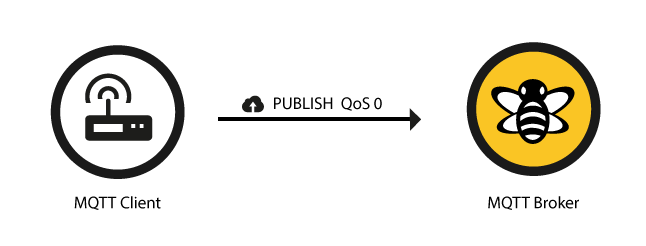
\includegraphics[scale=0.3]{images/qos0.png}
	\caption{MQTT QOS 0}
	\label{fig:mqtt0}
\end{figure}

	\item QOS 1 atau ``At least once” (gambar \ref{fig:mqtt1}), dimana pesan dikirim dengan jaminan setidaknya pesan sampai sekali ke tujuan. Sehingga memungkinkan terjadinya duplikasi pesan di tujuan akibat pesan yang dikirim ulang dari pengirim.
\begin{figure}[H]
	\centering
	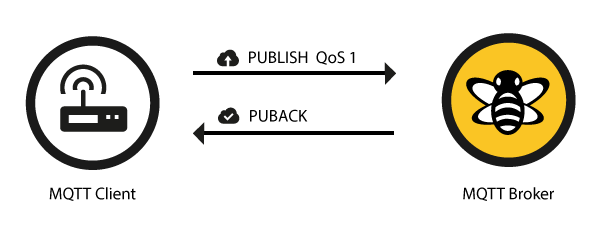
\includegraphics[scale=0.3]{images/qos1.png}
	\caption{MQTT QOS 1}
	\label{fig:mqtt1}
\end{figure}

	\item QOS 2 atau ``Exactly once" (gambar \ref{fig:mqtt2}), dimana pesan dikirm dengan jaminan diterima tepat sekali ke tujuan. Sehingga tidak ada pesan yang terduplikasi di tujuan.	
	
\begin{figure}[H]
	\centering
	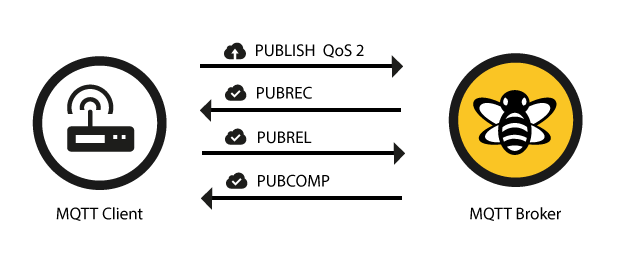
\includegraphics[scale=0.3]{images/qos2.png}	
	\caption{MQTT QOS 2}
	\label{fig:mqtt2}
\end{figure}
\end{enumerate}

\begin{figure}[H]
	\centering
	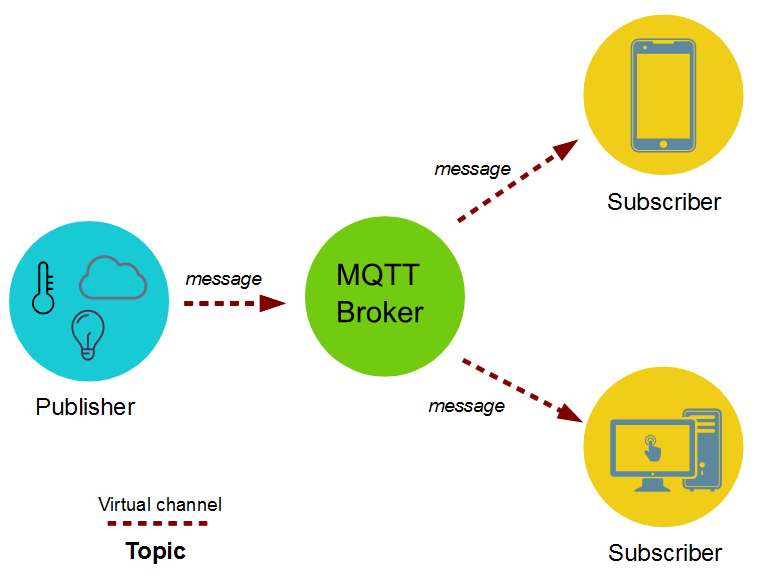
\includegraphics[scale=0.35]{images/mqtt.png}
	\caption{Cara kerja MQTT}
	\label{fig:how_mqtt}
\end{figure}

\section{Deteksi Puncak R oleh Pan and Tompkins}\label{bab2_pantom}
Pan dan Tompkins mengusulkan sebuah algoritma pencarian QRS pada sinyal ECG \cite{pantom}. Metode ini menjadi populer karena dapat bekerja secara \textit{real-time}. Metode PanTomkins dimulai dari proses processing berupa filtering sinyal. Kemudian dilanjutkan dengan pencarian puncak R menggunakan \textit{adaptive thresholding}. 

Pada tahap \textit{preprocessing}, Pan-Tompkins menerapkan 4 proses filtering yaitu Band Pass filtering, Derived filter, Squaring, dan Moving Window Integrator \ref{fig:preprocessing}. Tahapan tersebut dilakukan untuk menghilangkan \textit{noise} pada sinyal dan memudahkan proses pencarian puncak. 

Pada tahap processing, Pan-Tompkins menerapkan \textit{adaptive thresholding} terhadap sebuah window sinyal yang berukuran kecil (0.3s) \cite{pantom}. Pada window tersebut, akan dicari peak yang melewati threshold yang telah ditentukan, kemudian nilai peak akan menjadi input untuk  mengupdate nilai threshold. Ketika sekian waktu terlampaui tanpa ditemukannya peak maka harus dilakukan search back hingga posisi R terakhir yang ditemukan (gambar \ref{fig:processing_ori}).

\begin{figure}[htbp]
\centerline{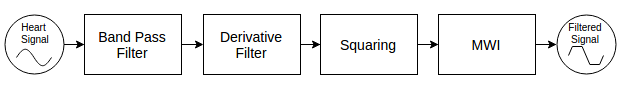
\includegraphics[scale=0.65]{images/preprocessing.png}}
\caption{Preprocessing: Filtering}
\label{fig:preprocessing}
\end{figure}

\begin{figure}[htbp]
\centerline{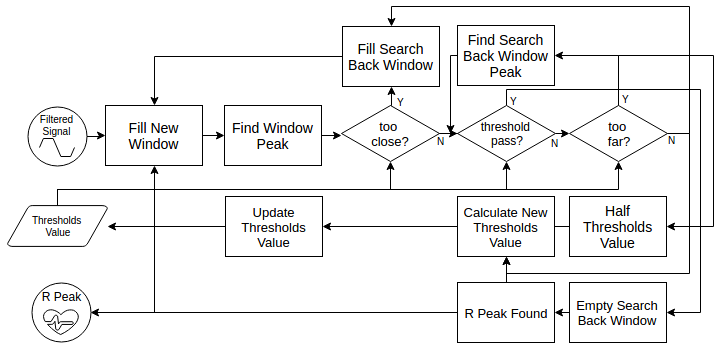
\includegraphics[scale=0.6]{images/processing_ori.png}}
\caption{Processing: Original R Peak Detection}
\label{fig:processing_ori}
\end{figure}

\section{Deteksi Aritmia oleh Tsipouras}\label{bab2_tsipouras}
Tsipouras et al. mengusulkan algoritma deteksi setelah melakukan percobaan bersama dokter spesialis jantung \cite{rr_classification}. Pada penelitiannya, ia membangun \textit{rule-based detector} berdasarkan masukan tim dokter jantung yang terlibat. \textit{Rule} ini dengan menggunakan sebuah (i) \textit{window RR-interval}, yang berisi 3 RR-interval, $RR1_i, RR2_i, RR3_i$. Jenis aritmia yang dapat dideteksinya dibagi menjadi 4 jenis detak aritmia dan 7 jenis ritme aritmia. Namun untuk rancangan pada paper ini artimia yang dapat dideteksi hanyalah jenis aritmia detak dan dikelompokkan kedalam 3 kategori. Kategori yang dipilih ialah 1) Normal, 2) Premature Contraction, dan 3) Ventricular Flutter. Secara detil pengelompokan ini dapat dilihat pada tabel \ref{table:beat_classification}.

\begin{table}[H]
\centering
	\begin{tabular}{|L{2cm}|L{8.5cm}|C{2cm}|}
	\hline
	\rowcolor{gray}
	\textbf{MIT-BIH Beat Symbol} & \textbf{Symbol Meaning} & 	\textbf{Category} \\
	\hline
	N & Normal & 1 \\
	. & Normal &  \\
	/ & Paced Beat & \\ 
	f & Fusion of paced and normal beat & \\
	L & Left bundle branch block & \\ 
	R & Right bundle branch block & \\ 
	x & Non-conducted P-wave (blocked Atrial Premature Contraction) & \\
	Q & Unclassifed & \\
	\hline
	V & Premature Ventricular Contraction & 2 \\
	A & Premature Atrial Contraction & \\
	a & Aberrated Premature Atrial Contraction & \\
	J & Nodal (junctional) premature beat & \\
	S & Supraventricular premature or ectopic beat (atrial or nodal) & \\
	F & Fusion of ventricular and normal beat & \\	
	\hline
	! & Ventricular Flutter & 3 \\
%	\hline
%	(BII & Heart block & 4 \\
	\hline
	\end{tabular}
	\caption{Pengelompokan Tipe beat}
	\label{table:beat_classification}
\end{table}

Algoritma Tsipouras melakukan klasifikasi berdasarkan sebuah window RR interval yaitu $RR1_i$, $RR2_i$, dan $RR3_i$ yang kemudian seterusnya bergeser satu beat. RR interval merupakan jaruk waktu antar puncak R dalam satu detak. Tiap beat mulanya dikategorikan sebagai kelas 1 dan kemudian mendapatkan kategori baru sesuai \textit{Rule} yang telah ditetapkan (gambar \ref{fig:flowchart_aritmia}).
\\
\\
Rule 1. VF: Dimulai ketika $RR1_i > 1.8RR2_i$ dan durasi $RR2_i$ lebih kecil daripada 0.6 s. Maka $RR2_i$ dianggap sebagai awal mula terjandinya VF dan window berikutnya akan dites dengan kedua kondisi berikut:

\begin{enumerate}
	\item durasi setiap RR interval dalam satu window lebih kecil dari 0.7s
	\item jumlah durasi setiap RR interval dalam satu window lebih kecil dari 1.7s
\end{enumerate}

Jika salah satu kondisi tambahan pada rule 1 terpenuhi minimal 4 window berurutan maka RR2 pada tiap window tersebut diklasifikasikan sebagai beat kategori 3. Jika tidak algoritma berlanjut dan window kembali ke posisi awal ditemukannya VF.
\\
\\
Rule 2. PVC: Detak dikategorikan sebagai PVC jika salah satu kondisi berikut terpenuhi:

\begin{enumerate}
	\item $RR1_i > 1.15RR2_i$ dan $RR3_i > 1.15RR2_i$
	\item $|RR1_i - RR2_i| < 0.3s$ dan $RR1_i < 0.8s$ dan $RR2_i < 0.8s$ dan $1.2(RR1_i + RR2_i)/2 < RR3_i$
	\item $|RR2_i$ - $RR3_i| < 0.3s$ dan $RR2_i < 0.8s$ dan $RR3_i < 0.8s$ dan $1.2(RR2_i + RR3_i)/2 < RR1_i$
\end{enumerate}

\begin{figure}[htbp]
\centerline{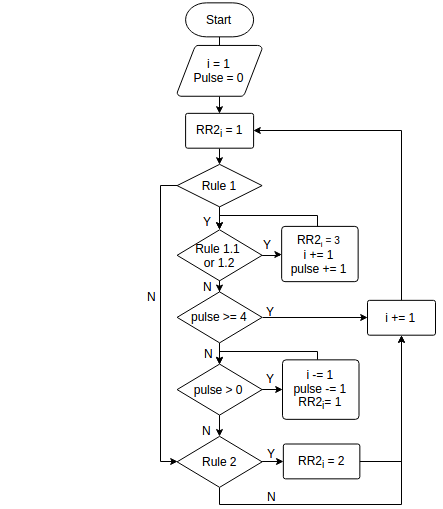
\includegraphics[scale=0.65]{images/flowchart_aritmia.png}}
\caption{Flowchart of Beat Aritmia Classification}
\label{fig:flowchart_aritmia}
\end{figure}

Pseudocode untuk flowchart deteksi aritmia (gambar \ref{fig:flowchart_aritmia}) dapat dilihat pada gambar \ref{algo:aritmia_rule}.

\begin{figure}[htbp]
	\centering
	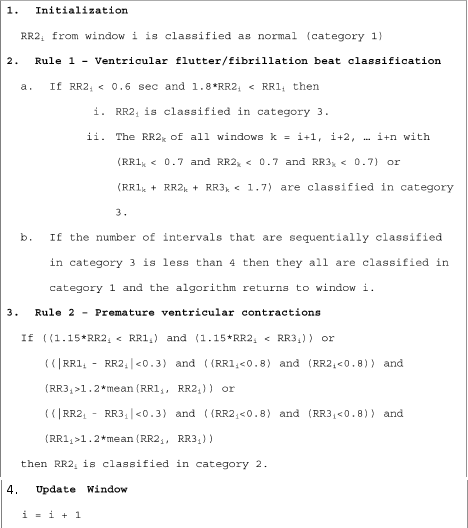
\includegraphics[scale=0.8]{images/algo_detect.png}
	\caption{Pseudo code algoritma yang diajukan Tsipouras}
	\label{algo:aritmia_rule}
\end{figure}